\documentclass[12pt,abstract]{scrartcl}
\usepackage{lipsum}
\usepackage{graphicx}

\title{Reproducible Science Template}
\author{Thomas Titscher, Christoph Pohl}
\date{\today}

\begin{document}

\maketitle

\begin{abstract}
  \lipsum[10]
\end{abstract}

\section{Introduction}

\lipsum[10]

\section{Methods}

Pure intuition.

\section{Results}

\begin{figure}[bt]
  \centering
  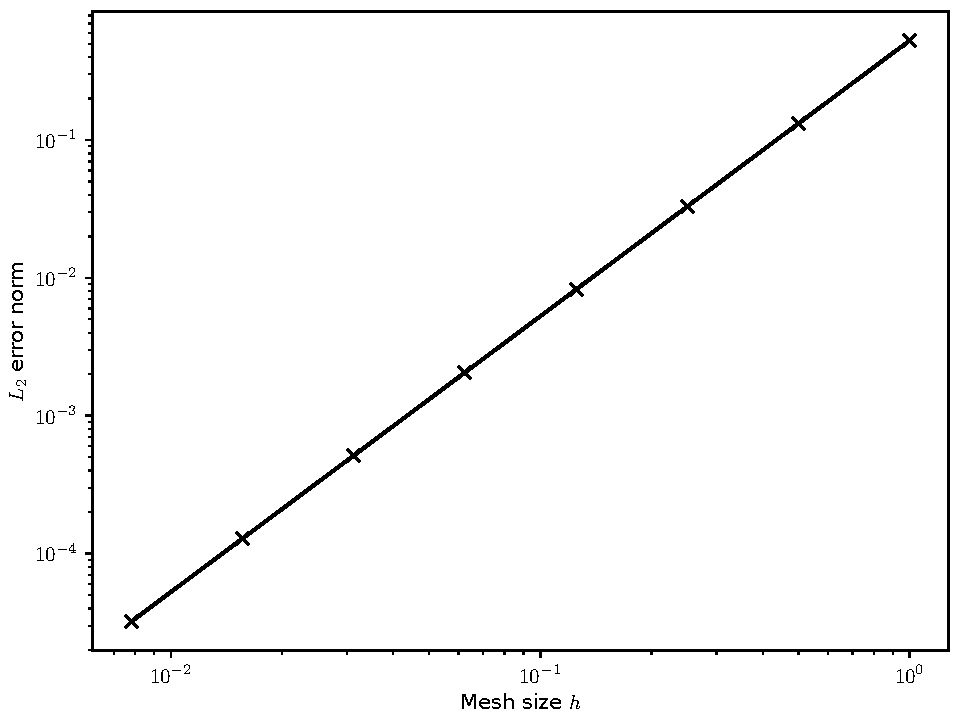
\includegraphics[width=0.6\linewidth]{poisson_convergence}
  \caption{Yip.}%
  \label{fig:poisson_convergence}
\end{figure}

\begin{figure}[bt]
  \centering
  \includegraphics[width=0.6\linewidth]{poisson_displacement_field}
  \caption{Yop.}%
  \label{fig:poisson_displacement_field}
\end{figure}

The results in Figure~\ref{fig:poisson_convergence} and Figure~\ref{fig:poisson_convergence} are impressive.

\end{document}
